\chapter{Appendix A}
\label{cha:Appendix A}



\section{Project Agreement}
\label{sec:Project Agreement}
\begin{figure}[H]
	\centering
        \framebox{
	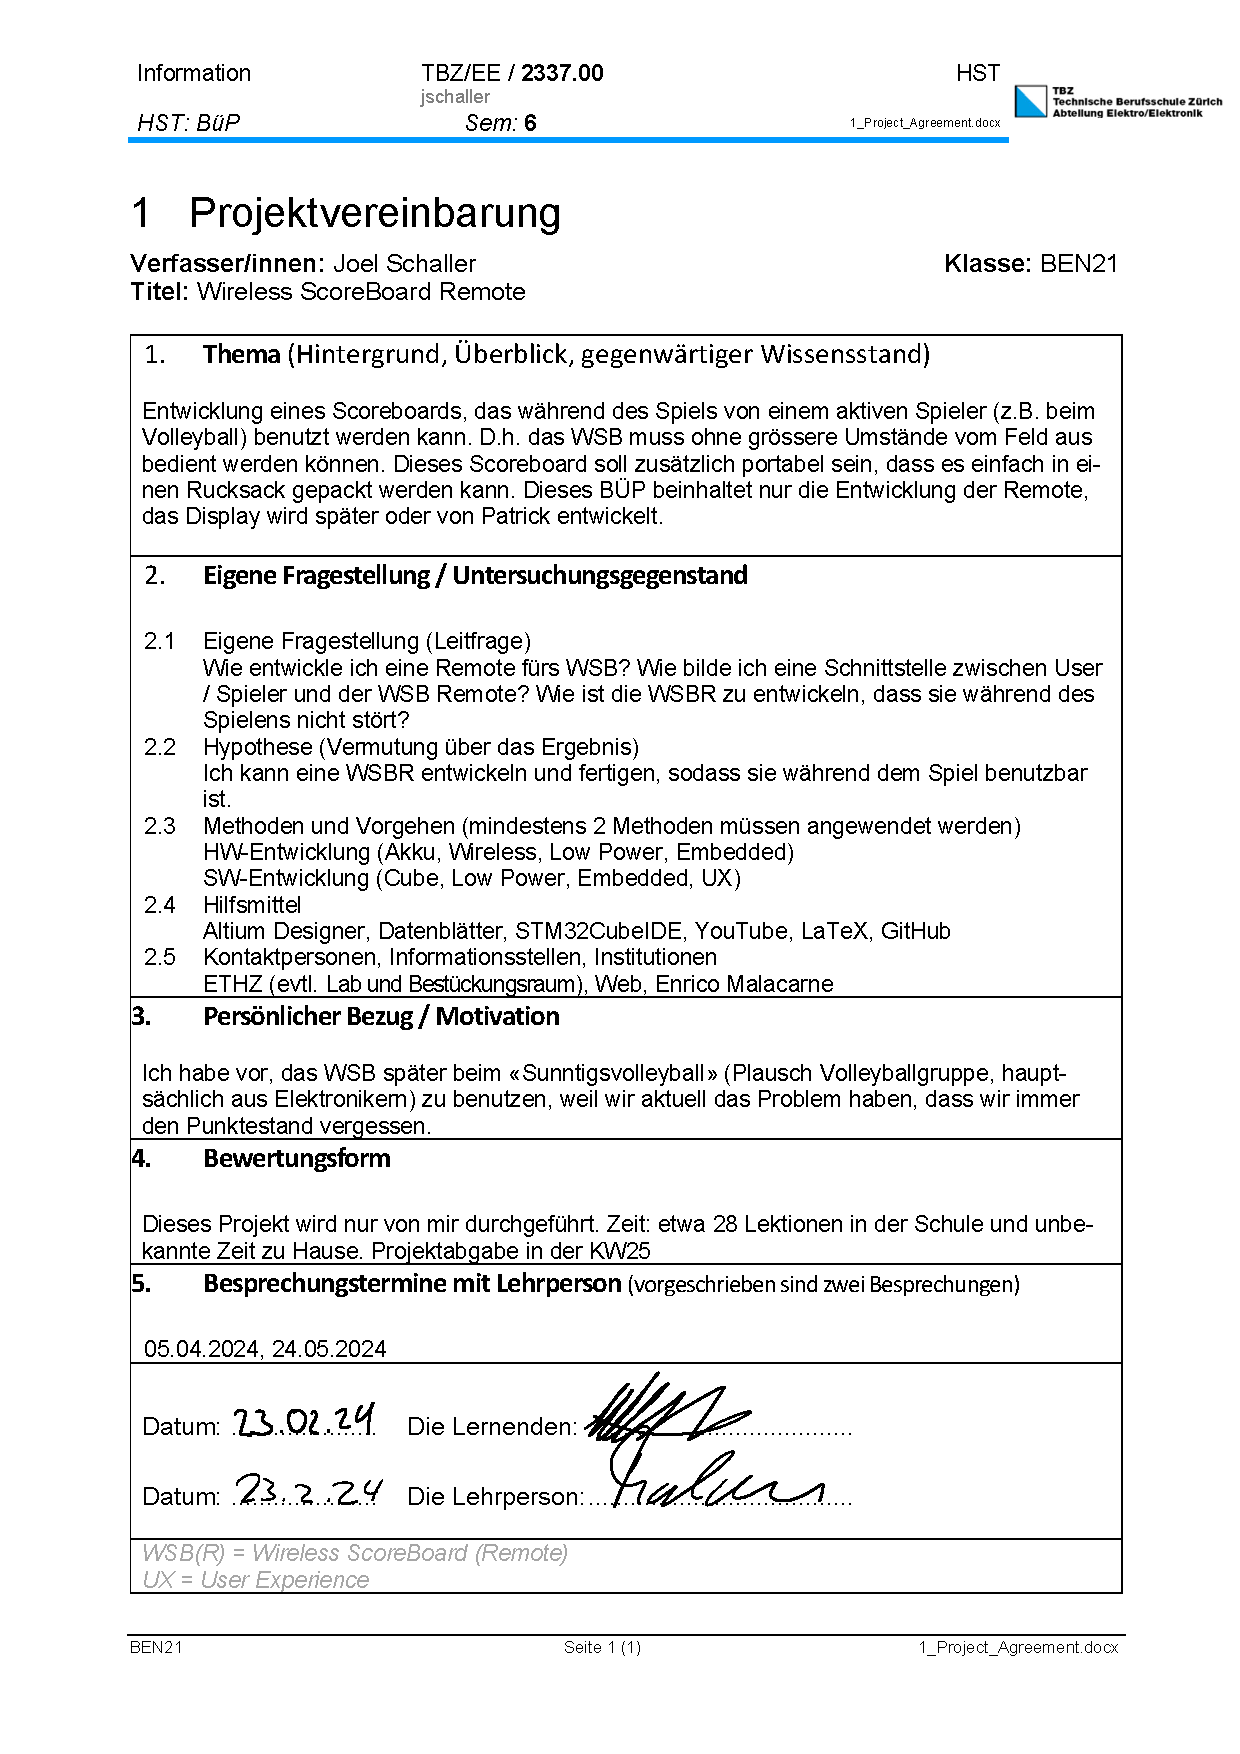
\includegraphics[width=14cm]{../../1_Agreement_Review/1_Project_Agreement.pdf}}
	\caption{Project Agreement}
	\label{fig:Project Agreement}
\end{figure}
\newpage


\section{Interview 1}
\label{sec:Interview 1}
\begin{figure}[H]
	\centering
        \framebox{
	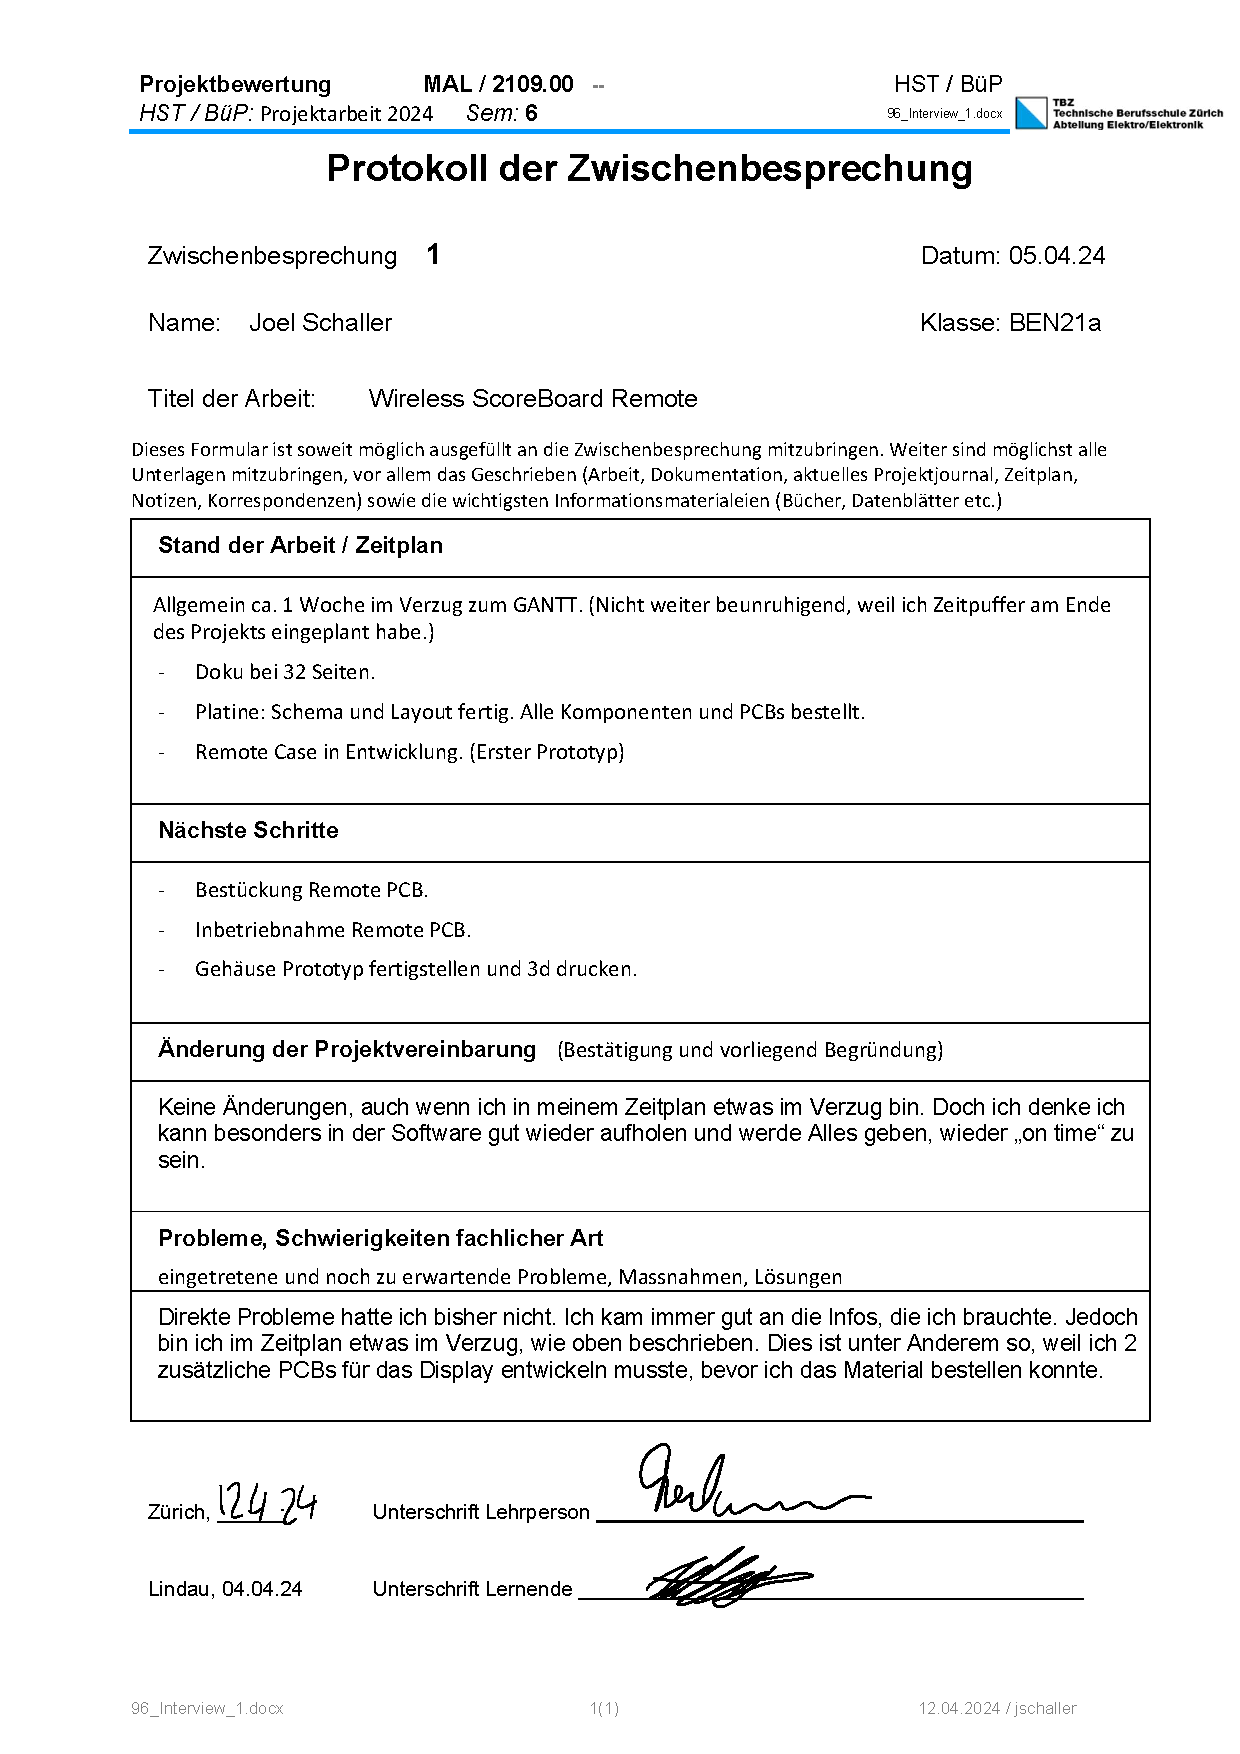
\includegraphics[width=15cm]{../../1_Agreement_Review/96_Interview_1.pdf}}
	\caption{Interview 1}
	\label{fig:Interview 1}
\end{figure}
\newpage


\section{GANTT}
\label{sec:GANTT}
\begin{figure}[H]
	\centering
        \framebox{
	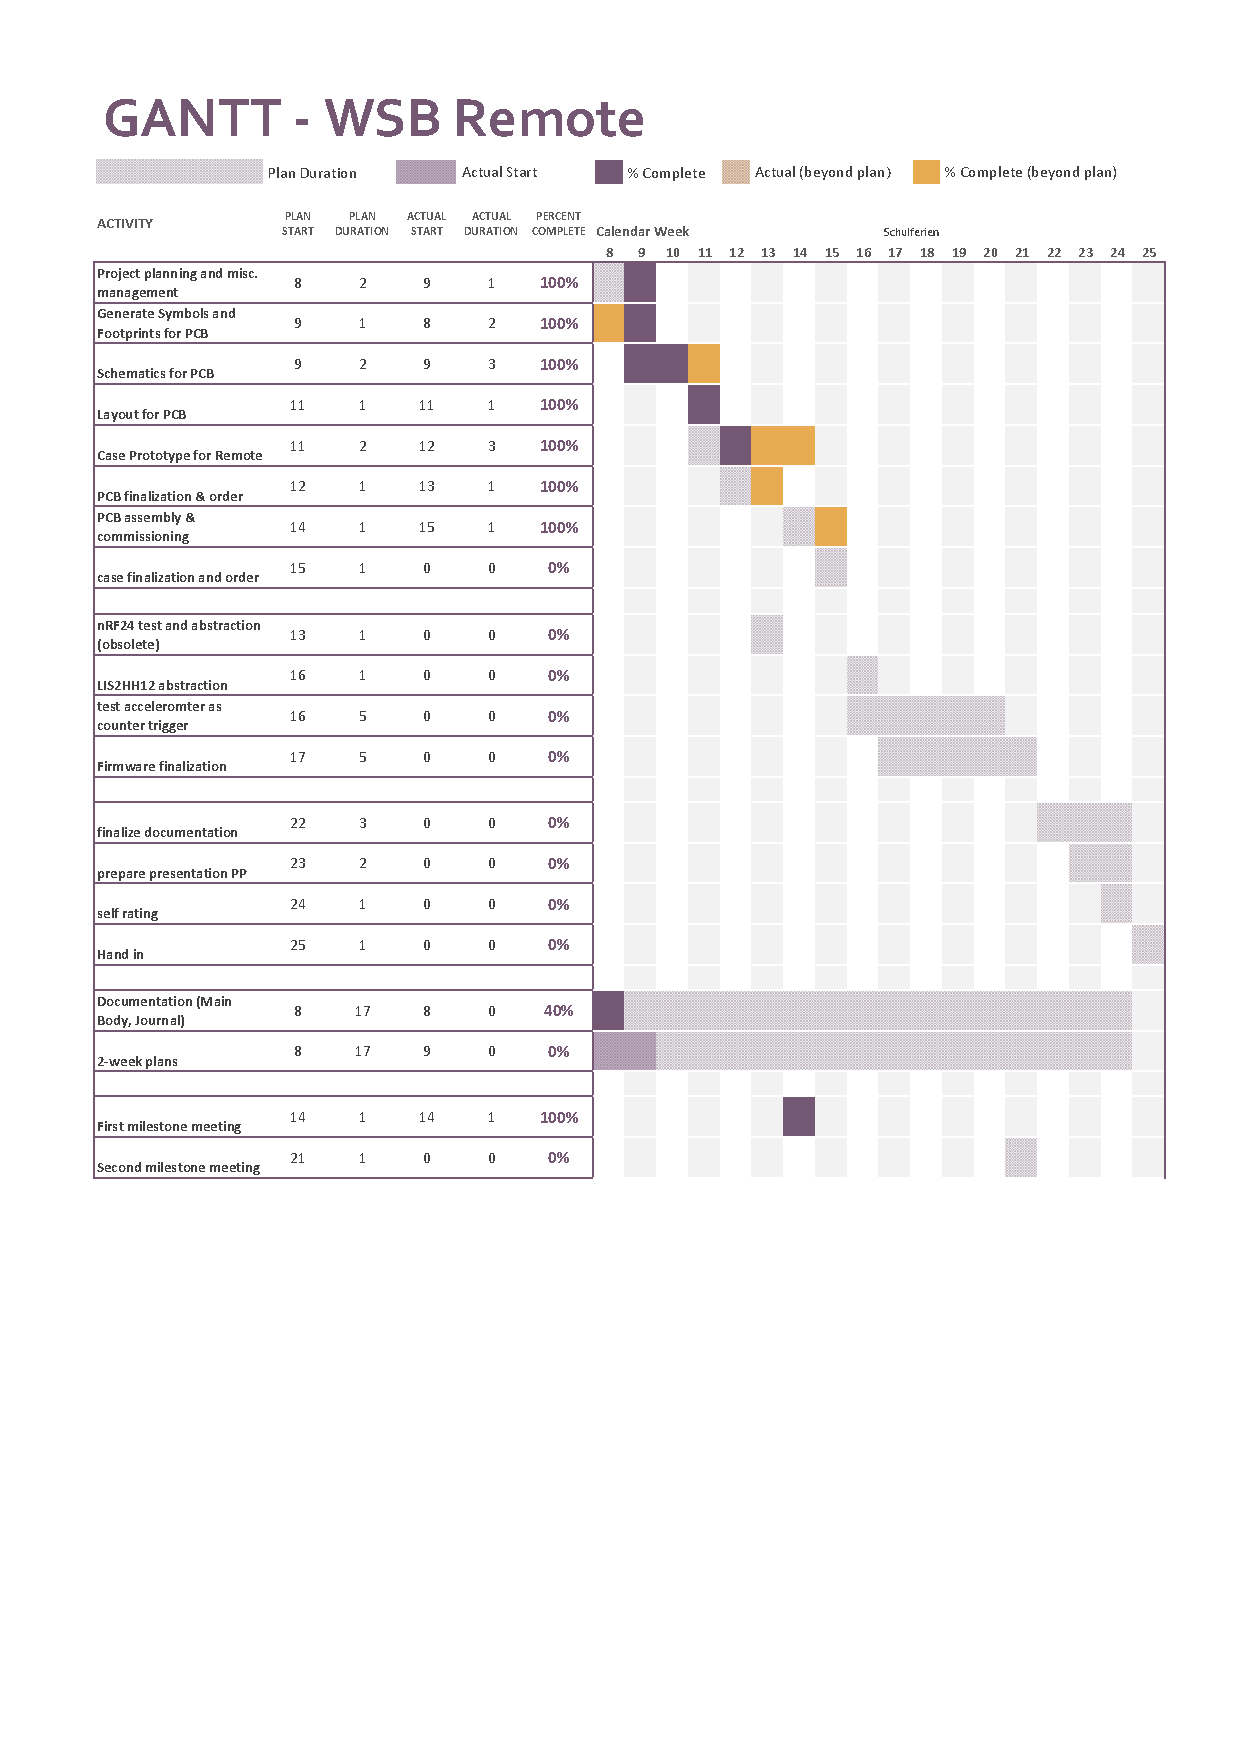
\includegraphics[width=14.5cm]{../GANTT/GANTT.pdf}}
	\caption{GANTT}
	\label{fig:GANTT}
\end{figure}



\section{2-week plans}
\label{sec:2-week plans}

\subsection{KW8 \& KW9}
\label{ssec:KW8_KW9}
\begin{itemize}
    \item Write and sign the project agreement.
    \item Add GANTT time planning diagram.
    \item Add project mindmap.
    \item Write "Pflichtenheft" and introduction.
    \item Draw all symbols and footprints for the remote PCB, that don't already exist in the Altium Vault.
    \item Maybe start with the schematics for the remote PCB.
    \begin{itemize}
        \item Microcontroller supply, SWD, Reset and misc. connections.
        \item Generate ioc file for microcontroller. (STM32Cube)
        \item Start with the power path schematics. (Battery, Battery Charger IC, Load Switch)
    \end{itemize}
\end{itemize}


\subsection{KW10 \& KW11}
\label{ssec:KW10_KW11}
\begin{itemize}
    \item Complete remote schematics.
    \begin{itemize}
        \item nRF24
        \item RGB LED
        \item accelerometer
        \item buttons
    \end{itemize}
    \item Prepare schematics and HW documentation for review.
    \item Ask Mr. Malacarne to review the remote schematics.
    \item Make the remote PCB layout.
    \item Start with the remote case prototype.
\end{itemize}


\subsection{KW12 \& KW13}
\label{ssec:KW12_KW13}
\begin{itemize}
    \item Order PCBs and Components.
    \item Design and 3d print a first case prototype.
\end{itemize}


\subsection{KW14 \& KW15}
\label{ssec:KW14_KW15}
\begin{itemize}
    \item Design and 3d print a first case prototype.
    \item Assembly and commissioning of WSBR board.
    \item Finalize WSBR Case and order it. (SLA translucent)
    \item First milestone meeting on 5th of April.
\end{itemize}


\subsection{KW16 \& KW17}
\label{ssec:KW16_KW17}
\begin{itemize}
    \item Finalize WSBR Case and order it. (SLA translucent)
    \item Define a standard for the communication between the remote and the display.
    \item BMS abstraction.
    \begin{itemize}
        \item Battery fuel gauge.
        \item Battery charging indicator.
        \item Turn on / off functions using the power button.
    \end{itemize}
    \item Accelerometer abstraction.
    \item Accelerometer as trigger tests and algorithm.
\end{itemize}


\subsection{KW18 \& KW19}
\label{ssec:KW18_KW19}
Holiday / language study trip Malta.


\subsection{KW20 \& KW21}
\label{ssec:KW20_KW21}
\begin{itemize}
    \item 
\end{itemize}


\subsection{KW22 \& KW23}
\label{ssec:KW22_KW23}
\begin{itemize}
    \item 
\end{itemize}


\subsection{KW24 \& KW25}
\label{ssec:KW24_KW25}
\begin{itemize}
    \item 
\end{itemize}
\newpage




\section{Journal}
\label{sec:Journal}
\begin{table}[H]
    \centering
\begin{tabular}{||c | c | c || c||} 
 \hline
 Date &  Location & Dur. & Activity \\ [0.5ex] 
 \hline\hline
    30.01.2024 & HOME & 2h & Set up GitHub repo and documentation \\   
 \hline
    01.02.2024 & HOME & 0.5h & First draft of project agreement [\ref{sec:Project Agreement}] \\ 
 \hline
    17.02.2024 & HOME & 3h & Acc test as counter trigger [\ref{sec:Trigger}] \\ 
 \hline
    18.02.2024 & HOME & 0.5h & doc: acc test results [\ref{ssec:Accelerometer}] \\ 
 \hline
    18.02.2024 & HOME & 1h & battery charging: R\&D [\ref{sec:Battery Charging}] \\ 
 \hline
    18.02.2024 & HOME & 2h & HW Concept [\ref{sec:HW Concept}] \\ 
 \hline
    19.02.2024 & HOME & 2.5h & Started drawing SYM and FP for WSBR Schematic \\ 
 \hline
    23.02.2024 & TBZ & 0.5h & Signed Project Agreement [\ref{sec:Project Agreement}] \\ 
 \hline
    26.02.2024 & HOME & 1.5h & Project Mindmap [\ref{sec:Mindmap}] / GANTT [\ref{sec:GANTT}] \\ 
 \hline
    27.02.2024 & HOME & 0.5h & Bought LiPo battery / 2-week plan KW8 \& KW9 [\ref{ssec:KW8_KW9}] \\ 
 \hline
    28.02.2024 & HOME & 0.5h & Added some components to remote schematics [\ref{sec:Schematics}] \\ 
 \hline
    29.02.2024 & HOME & 1h & Added missing components \& Added missing datasheets \\ 
 \hline
    01.03.2024 & TBZ & 1h & Added missing components \& Added missing datasheets \\ 
 \hline
    01.03.2024 & HOME & 1.5h & "Pflichtenheft" \& Init ioc file \& Added missing comp. \\ 
 \hline
    02.03.2024 & HOME & 2h & MCU pinout \& Schem: MCU, SWD, USBC [\ref{sec:Schematics}] \\ 
 \hline
    03.03.2024 & HOME & 2h & Drawn power section schematics [\ref{sec:Schematics}] \\ 
 \hline
    04.03.2024 & HOME & 1h & Drawn: nRF, acc, LEDs, BTs [\ref{sec:Schematics}] \\ 
 \hline
    06.03.2024 & HOME & 2.5h & Completed schematics and self-review [\ref{sec:Schematics}] \\ 
 \hline
    07.03.2024 & HOME & 1h & doc: Schematics battery management [\ref{ssec:Schematics}] \\ 
 \hline
     08.03.2024 & TBZ & 1.5h & remote schematics review with Mr. Malacarne [\ref{ssec:Remote Schematics Review}] \\ 
 \hline
     11.03.2024 & HOME & 1h & documented review [\ref{ssec:Remote Schematics Review}] \& found new RF module [\ref{sssec:RF module switch}] \\ 
 \hline
     12.03.2024 & HOME & 3h & made (schematic) changes from review. \\ 
 \hline
     13.03.2024 & HOME & 0.25h & Written: HC\_12 in [\ref{sssec:RF module switch}] \\ 
 \hline
     13.03.2024 & HOME & 2.5h & PCB: General placement \\ 
 \hline
     14.03.2024 & HOME & 1.5h & PCB: layed out components. \\ 
 \hline
     15.03.2024 & TBZ & 1h & Doc: Vibration motor decision, HC\_12\\ 
 \hline
     16.03.2024 & HOME & 1.5h & done component layout. \\ 
 \hline
     17.03.2024 & HOME & 3h & WSBR Board routing. \\ 
 \hline
     17.03.2024 & HOME & 2h & WSBR Board V1.1 done. \\ 
 \hline
     23.03.2024 & HOME & 1h & Started WSBR prototype. \\ 
 \hline
     30.03.2024 & HOME & 2h & wip WSBR Case. \\ 
 \hline
\end{tabular}
    \caption{Project Journal 1}
    \label{tab:Project Journal 1}
\end{table}




\begin{table}[H]
    \centering
\begin{tabular}{||c | c | c || c||} 
 \hline
 Date &  Location & Dur. & Activity \\ [0.5ex] 
 \hline\hline
     31.03.2024 & HOME & 1h & Ordered components and PCB. \\ 
 \hline
     11.04.2024 & ETH & 1h & WSBR Case prototype finalization and 3d printing. \\ 
 \hline
     11.04.2024 & ETH & 2.5h & Population WSBR PCB. (Vapour-phase and stencil)\\ 
 \hline
     12.04.2024 & TBZ & 1.5h & documentation WIP. \\ 
 \hline
     13.04.2024 & HOME & 2h & case finalization \& start commissioning. \\ 
 \hline
     14.04.2024 & HOME & 1h & commissioning WIP. \\ 
 \hline
     24.04.2024 & ETH & 3.5h & commissioning done, accelerometer dead-bug modification \\ 
 \hline
     24.04.2024 & HOME & 0.5h & ordered translucent WSBR case. \\ 
 \hline
     25.04.2024 & HOME & 1.5h & FW: BMS functions \& intro of all lib files. \\ 
 \hline
\end{tabular}
    \caption{Project Journal 2}
    \label{tab:Project Journal 2}
\end{table}
